%====================================================================
\subsection{Network inference}
%====================================================================
\frame{\frametitle{Network inference} \pause

  \bigskip
  \paragraph{Distinguishing between direct and indirect interactions.}
  \begin{itemize}
    \setlength{\itemsep}{0.5\baselineskip}
    \item The variations of species abundance can be all correlated,
    \item Some correlations result from 'direct' interactions ($A$ eats $B$). 
    \item Some others result from 'indirect' interactions  (both $A$ and $B$ are preys of $C$).
  \end{itemize}
   \pause \medskip
  \ra Probabilistic translation: \emphase{\sl conditional} dependence vs \emphase{\sl marginal} dependence.

  \pause \bigskip \bigskip
  \paragraph{Graphical model} encodes the dependency structure into a graph $G$ in which only conditionally {\sl dependent variables} are connected.
  
  \pause \bigskip \bigskip \bigskip
  \begin{tabular}{cc}
    \hspace{-.04\textwidth}
    \begin{tabular}{p{.65\textwidth}}
      \paragraph{Example:}
      \begin{itemize}
        \setlength{\itemsep}{0.5\baselineskip}
        \item All variables (species) are dependent
        \item But 4 is independent from 1 and 2 conditionally on 3 \\ ~
        \item \textcolor{gray}{Formally: $p(y_1, y_2, y_3, y_4) \propto \psi_1(y_1, y_2, y_3) \psi_2(y_3, y_4).$}
      \end{itemize}
      \bigskip \bigskip ~
    \end{tabular}
    &
    \begin{tabular}{p{.25\textwidth}}
      \hspace{-.1\textwidth}
      \includegraphics[width=.3\textwidth, trim=90 90 50 90, clip=]{\fignet/FigGGM-4nodes}
    \end{tabular}
  \end{tabular}

}

%====================================================================
\frame{\frametitle{Network inference in the PLN model} \pause

  \bigskip
  \paragraph{PLN model.} The dependency is encoded in the Gaussian latent layer, with covariance matrix $\Sigma$.
  
  \pause \bigskip \bigskip
  \paragraph{Gaussian case.} The graph $G$ of direct interactions is given by the precision matrix
  $$
  \Omega = \Sigma^{-1}
  $$
  ({\sl partial} correlations vs {\sl marginal} correlations).
  
  \pause \bigskip \bigskip \bigskip 
  \begin{tabular}{cc}
    \hspace{-.04\textwidth}
    \begin{tabular}{p{.6\textwidth}}
      \paragraph{PLN version.} \refer{CMR19}
      \medskip
      \begin{itemize}
        \setlength{\itemsep}{1\baselineskip}
        \item Fit a PLN model, forcing $\Omega = \Sigma^{-1}$ to be sparse.
        \item Algorithm similar to the graphical lasso \refer{FHT08}. \\ ~
        \item \pause The sparsity of $\Omega$ is tuned via a penalty parameter $\lambda$.
        \item $\lambda$ can be chosen via standard criteria (BIC, ...).
      \end{itemize}
      \bigskip \bigskip ~
    \end{tabular}
    &
    \hspace{-.05\textwidth}
    \begin{tabular}{p{.4\textwidth}}
      \includegraphics[height=.5\textheight, trim=25 5 10 0, clip=]{\fignet/BarentsFish_Gfull_criteria}
    \end{tabular}
  \end{tabular}

}

%====================================================================
\frame{\frametitle{Barents' fish} 
  
  \vspace{-.05\textheight}
  \begin{tabular}{cc}
    \hspace{-.04\textwidth}
    \begin{tabular}{p{.22\textwidth}}
      \paragraph{Data:} \\ ~
      \begin{itemize}
      \item $n=89$ sites \\~
      \item $p=30$ species \\~
      \item $d=4$ covariates
        \begin{itemize}
        \item latitude
        \item longitude
        \item temperature
        \item depth
        \end{itemize}
      \end{itemize}
    \end{tabular}
    &
    \begin{tabular}{c}
      \includegraphics[height=.85\textheight]{\fignet/CMR18b-ArXiv-Fig5}
    \end{tabular}
  \end{tabular}
  }

%====================================================================
\frame{\frametitle{Oak powdery mildew}

  \begin{tabular}{cc}
    \hspace{-.04\textwidth}
    \begin{tabular}{p{.35\textwidth}}
      \paragraph{Network inference.} \refer{JFS16} ~
      
      \bigskip
      {\sl Erysiphe alphitoides} (Ea) = \\
      ~ \\
      fungus reponsible for the disease
    \end{tabular}
    &
%     \hspace{-.075\textwidth}
    \begin{tabular}{p{.65\textwidth}}
      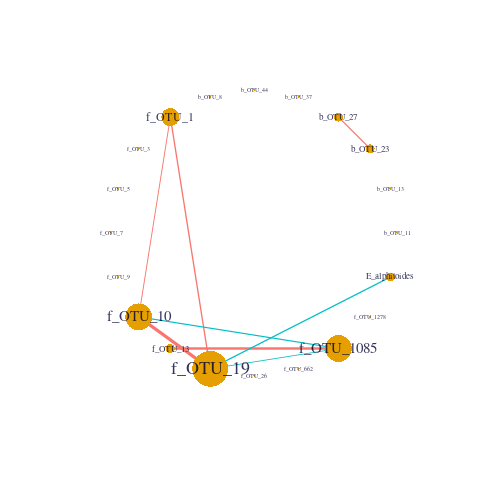
\includegraphics[height=.7\textheight, trim=50 50 50 50, clip=]{\fignet/Oaks-p20-network}
    \end{tabular}
  \end{tabular}

  
  \pause \bigskip
  \ra See also tree-based network inference, including {\sl missing actors} \refer{SRS19,MRA20,MRA21}
}

